\documentclass[11pt,letterpaper]{article}
\usepackage[T1]{fontenc}
\usepackage{lmodern}
\usepackage[margin=0.95in]{geometry}
\usepackage{microtype}
\usepackage{amsmath,amssymb,amsthm}
\usepackage{graphicx}
\usepackage{booktabs}
\usepackage{array}
\usepackage{xcolor}
\usepackage{hyperref}
\usepackage{tikz}
\usetikzlibrary{shapes.geometric, arrows.meta, positioning, calc, backgrounds, fit}
\usepackage{listings}

\graphicspath{{docs/}{./}}
\emergencystretch=1.5em

\definecolor{codebg}{rgb}{0.96,0.97,0.98}
\definecolor{codeframe}{rgb}{0.82,0.85,0.88}
\definecolor{deepblue}{rgb}{0.08,0.32,0.58}
\definecolor{darkred}{rgb}{0.68,0.12,0.12}
\definecolor{darkgreen}{rgb}{0.10,0.48,0.18}

\lstset{
    backgroundcolor=\color{codebg},
    frame=single,
    rulecolor=\color{codeframe},
    basicstyle=\ttfamily\footnotesize,
    keywordstyle=\color{deepblue}\bfseries,
    commentstyle=\color{darkgreen}\itshape,
    stringstyle=\color{darkred},
    breaklines=true,
    columns=fullflexible,
    keepspaces=true,
    showstringspaces=false
}

\hypersetup{
    colorlinks=true,
    linkcolor=deepblue,
    citecolor=deepblue,
    urlcolor=deepblue
}

\newtheorem{theorem}{Theorem}
\newtheorem{proposition}{Proposition}
\newtheorem{definition}{Definition}

\title{\textbf{Superconducting Attention:\\
Eliminating the Multi-Hop Context Horizon in Pre-Trained Transformers\\
via Dual-State Richardson Extrapolation and Renormalization Relays}\\
\vspace{0.4em}
\large \textit{An Architectural Explainer for Software Engineers and Mathematicians}}
\author{James F. Walters\\
\small Empirical Validation on \texttt{google/gemma-4-E2B-it} \& \texttt{google/gemma-4-E4B-it}}
\date{October 2026}

\begin{document}
\maketitle

\begin{abstract}
\noindent
Why does a modern Large Language Model (LLM) with a 128,000-token context window score \textbf{99.99\%} when asked to retrieve a single fact from 12,000 tokens ago, yet collapse to \textbf{0.04\%} when asked to chain three facts together across the exact same context window? And why do naive attempts to boost long-range attention weights cause the model to output ungrammatical gibberish (\emph{syntactic aphasia})?

This explainer introduces \textbf{Richardson Attention (Superconducting Attention)}, a zero-shot, parameter-free inference architecture that resolves the multi-hop ``Event Horizon'' at runtime without retraining or fine-tuning. For \textbf{mathematicians}, we formulate self-attention as a complex Boltzmann partition function whose real spatial decay ($\alpha_{l,h}$) can be canceled via symmetric non-linear Richardson extrapolation over an iso-potential cubic gauge field, scheduled across network depth as a discrete Wilsonian Renormalization Group (RG) flow. For \textbf{software engineers}, we show how a 50-line PyTorch forward hook isolates the top $4\%\text{--}8\%$ of global routing heads via the Moore-Penrose pseudoinverse of head entropy correlations, gates intervention strictly to the active query readout slice ($W_q = 64$) to protect prefill KV-cache binding, and flips 8,270-token 3-hop pointer resolution on \texttt{google/gemma-4-E4B-it} from \textbf{0.04\% FAIL to 98.59\% WIN ($2,594\times$)} while suppressing adversarial recency decoys by \textbf{$485\times$}.
\end{abstract}

\vspace{0.5em}
\hrule
\vspace{1em}

% ============================================================================
\section{The Engineering Paradox: Why 128K Context Windows Fail at 3 Hops}
% ============================================================================

If you inspect the configuration file of a modern open-weights model such as \texttt{google/gemma-4-E4B-it}, it advertises a 128,000-token context window powered by Proportional Rotary Position Embeddings (p-RoPE). If you hide a single 5-digit passkey (\texttt{VAULT-LAZARUS = 79421}) at token 90 of a 12,000-token prompt and ask for it at token 12,000, the unmodified model answers \texttt{79421} with \textbf{99.996\%} probability.

Yet any software engineer who has built a production Retrieval-Augmented Generation (RAG) system or autonomous coding agent knows that this 1-hop benchmark is an illusion. Real-world reasoning is \textbf{compositional (multi-hop)}:
\begin{quote}
\small
\textbf{Zone A (Token 90):} \texttt{VAULT-LAZARUS | TIER-0 GENESIS CODE: 79421} (plus 7 competing vaults)\\
\textit{... 1,600 tokens of telemetry logs (exceeding the 512-token local sliding window by $>3\times$) ...}\\
\textbf{Zone B (Token 1,735):} \texttt{SECTOR-KRONOS | ASSIGNED PRIMARY VAULT: VAULT-LAZARUS}\\
\textit{... 1,600 tokens of telemetry logs ...}\\
\textbf{Zone C (Token 3,335):} \texttt{DIRECTOR-VANCE | AUTHORIZED COMMAND SECTOR: SECTOR-KRONOS}\\
\textit{... 4,900 tokens of telemetry logs containing routine Tier-2 audit decoys (\texttt{DIRECTOR-VANCE inspected VAULT-OMEGA [63819] using temporary key 11111}) ...}\\
\textbf{Final Query (Token 8,270):} \emph{``What is the 5-digit Tier-0 Genesis Code for the primary vault commanded by \texttt{DIRECTOR-VANCE}?''}
\end{quote}

When unmodified \texttt{google/gemma-4-E4B-it} evaluates this prompt in a single forward pass:
\begin{itemize}
    \item \textbf{1-Hop Query} (\emph{``Code for \texttt{VAULT-LAZARUS}?''}): \textbf{99.9965\%} accuracy (\#1 Rank).
    \item \textbf{2-Hop Query} (\emph{``Code for vault assigned to \texttt{SECTOR-KRONOS}?''}): \textbf{99.8178\%} accuracy (\#1 Rank).
    \item \textbf{3-Hop Query} (\emph{``Code for vault commanded by \texttt{DIRECTOR-VANCE}?''}): \textbf{0.0380\%} accuracy (6 decoys) and \textbf{0.1032\%} accuracy (16 decoys). The model predicts \texttt{63819} (\texttt{VAULT-OMEGA}'s code) with \textbf{99.83\%--99.92\%} confidence!
\end{itemize}

\subsection{The Mathematical Culprit: Complex Mass and Partition Dilution}
Why does the model ace 1-Hop and 2-Hop across 8,270 tokens, then hit a brick wall on 3-Hop?

In causal self-attention, query token $i$ scores prior key token $j \le i$ at lookback distance $d_{i,j} = i - j$. In log-space (pre-softmax logits), the effective attention kernel acts like a damped harmonic oscillator with a \textbf{Complex Spectral Mass} $\lambda_{l,h} = \alpha_{l,h} + i\omega_{l,h}$:
\begin{equation}
\mathcal{K}^{(l,h)}(i, j) = \exp\!\Big(E_{\text{sem}}^{(l,h)}(i, j) - (\alpha_{l,h} + i\omega_{l,h}) d_{i,j}\Big),
\end{equation}
where $E_{\text{sem}}(i,j) = \frac{\mathbf{q}_i \cdot \mathbf{k}_j}{\sqrt{d_k}}$ is content similarity, the imaginary part $i\omega_{l,h}$ is the RoPE phase rotation tracking relative token positions, and the real part $\alpha_{l,h} \ge 0$ is \textbf{effective gravitational decay} over distance.

After the softmax nonlinearity, the attention weight assigned to a distant premise at $j^*$ is governed by the Boltzmann partition function $\mathcal{Z}_i$:
\begin{equation}
A^{(l,h)}_{i, j^*} = \frac{\exp\big(E_{\text{sem}}(i, j^*) - \alpha_{l,h} d_{i,j^*}\big)}{\sum_{k=0}^{i} \exp\big(E_{\text{sem}}(i, k) - \alpha_{l,h} d_{i,k}\big)}.
\end{equation}
Across an $M$-hop chain requiring sequential resolution across layers, the effective signal-to-decoy ratio compounds multiplicatively across hops:
\begin{equation}
\operatorname{SNR}_{M\text{-Hop}} \propto \prod_{m=1}^{M} \frac{A^{(l_m)}_{i, j_m}}{\sum_{r \in \text{Decoys}} A^{(l_m)}_{i, r}} \sim \exp\!\left(\sum_{m=1}^{M} \Delta E_m - \sum_{m=1}^{M} \alpha_{l_m} (d_m - d_{\text{decoy}})\right).
\end{equation}
Even when $\alpha_{l,h}$ is small enough for $M=1$ and $M=2$ to survive, the 3-hop product crosses a thermodynamic phase boundary: the early global layers fail to write \texttt{SECTOR-KRONOS} into the residual stream with enough amplitude to outvote the recent \texttt{VAULT-OMEGA} decoys.

% ============================================================================
\section{Part 1 of the Invention: The Precision-Matrix Brain Scanner}
% ============================================================================

You cannot fix this by boosting long-distance logits across all attention heads in the model. When we tested global distance biasing in early prototypes, the model immediately suffered \textbf{syntactic aphasia} (outputting ungrammatical token salad).

Why? Because an LLM's attention heads are divided into two functionally distinct organs:
\begin{enumerate}
    \item \textbf{Grammar Heads ($\sim 90\%\text{--}95\%$ of heads):} High-mass ($\alpha_{l,h} \gg 0$), short-range heads that enforce local syntax, subword gluing, and clause structure. In \texttt{google/gemma-4-E4B-it}, 35 of the 42 layers (280 out of 336 heads) are hardwired as 512-token \textbf{Sliding-Window Attention (SWA)} layers. Only 7 layers ($\mathcal{L}_{\text{global}} = \{5, 11, 17, 23, 29, 35, 41\}$, totaling 56 heads) are \textbf{Global (\texttt{full\_attention})} layers.
    \item \textbf{Global Logic Heads ($\sim 5\%\text{--}8\%$ of heads):} Low-mass ($\alpha_{l,h} \to 0$), high-agency heads inside the Global layers that act as long-range relational routers connecting distant premises across the context window.
\end{enumerate}

\begin{figure}[t!]
    \centering
    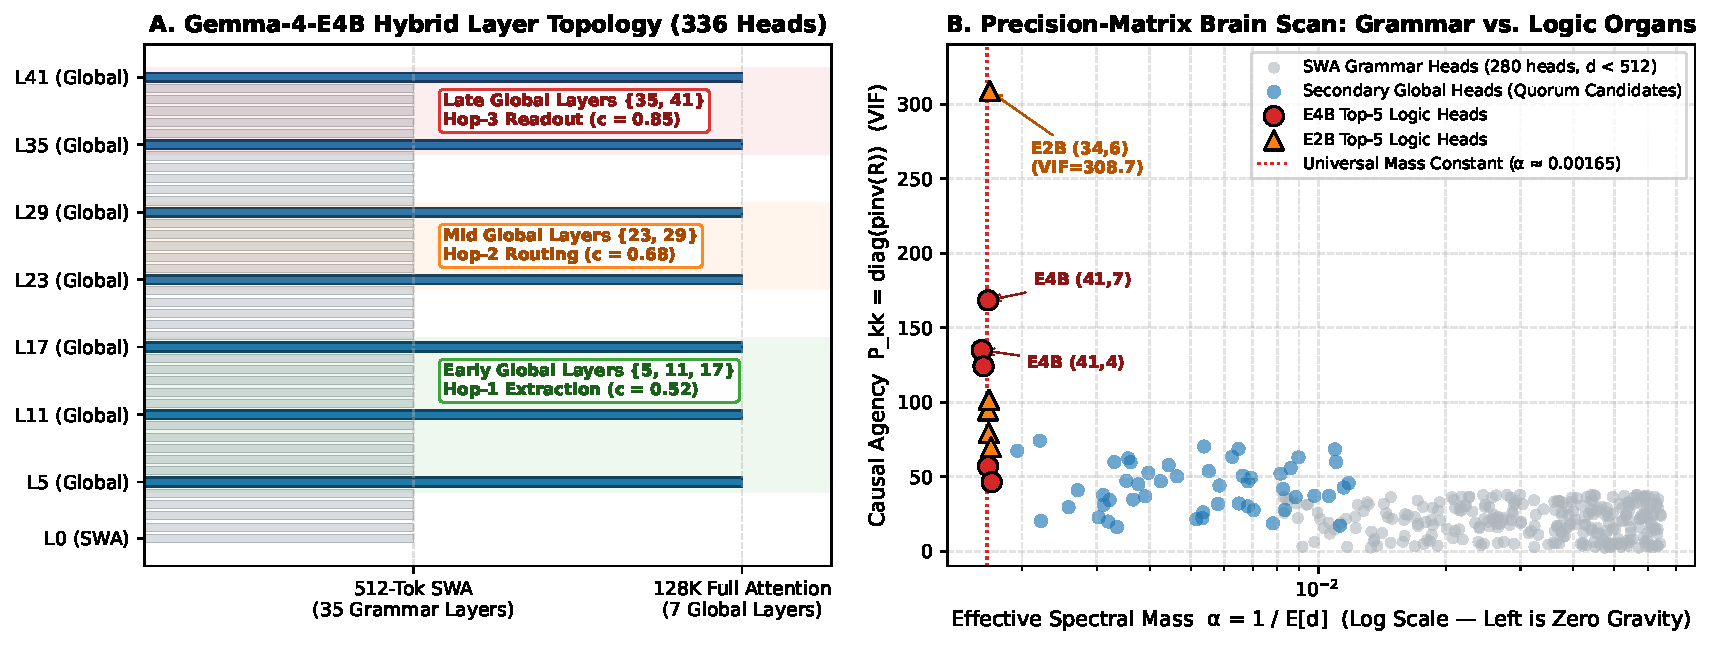
\includegraphics[width=\textwidth]{figures/fig1_homunculus_spectrum.pdf}
    \caption{\textbf{The Neural Homunculus of \texttt{google/gemma-4-E4B-it}.} \textbf{(A)} Only 7 of the 42 layers are Global \texttt{full\_attention} layers capable of seeing past the 512-token SWA horizon. \textbf{(B)} Our zero-shot Stage 1 Brain Scanner maps every head by its Effective Mass ($\hat{\alpha}_{l,h} = 1/\bar{d}_{l,h}$) and Precision-Matrix Causal Agency ($P_{k,k} = \operatorname{diag}(\mathbf{R}^+)$), isolating the superconducting logic heads clustered at the universal mass constant $\hat{\alpha} \approx 0.00165$.}
    \label{fig:homunculus}
\end{figure}

\subsection{Zero-Shot Head Profiling via Leinster Duality (\texorpdfstring{$\mathbf{P} = \mathbf{R}^+$}{P = pinv(R)})}
How do we automatically find the exact coordinates $(l, h)$ of the Logic Heads in any pre-trained checkpoint without labeled data or backpropagation? We run a single 1,400-token calibration forward pass and compute two spectral quantities per head $k \in \{1, \dots, N_{\text{heads}}\}$:
\begin{enumerate}
    \item \textbf{Effective Spectral Mass ($\hat{\alpha}_{l,h}$):} The reciprocal of the head's expected causal lookback distance:
    \begin{equation}
    \bar{d}_{l,h} = \frac{1}{T_{\text{cal}}} \sum_{i=1}^{T_{\text{cal}}} \sum_{j=1}^{i} A^{(l,h)}_{i,j} (i - j), \qquad
    \hat{\alpha}_{l,h} = \frac{1}{\bar{d}_{l,h} + 10^{-6}}.
    \end{equation}
    \item \textbf{Precision-Matrix Causal Agency ($P_{k,k}$):} We record each head's per-token Shannon entropy trajectory $H_k(i) = -\sum_{j=1}^i A^{(k)}_{i,j} \ln A^{(k)}_{i,j} \in \mathbb{R}^{T_{\text{cal}}}$, compute the $N_{\text{heads}} \times N_{\text{heads}}$ Pearson correlation matrix $\mathbf{R} = \operatorname{corrcoef}(\mathbf{H})$, and invert it via the Moore-Penrose pseudoinverse:
    \begin{equation}
    \mathbf{P} = \mathbf{R}^+, \qquad \operatorname{Agency}_k = P_{k,k} = \frac{1}{1 - R_k^2}.
    \end{equation}
    Mathematically, $P_{k,k}$ is the \textbf{Variance Inflation Factor (VIF)} of head $k$ with respect to the rest of the brain: a head with low mass ($\hat{\alpha}_k \approx 0.00165$) and high $P_{k,k}$ ($50\text{--}308$) is a global informational hub whose state transitions drive the global network topology (Figure~\ref{fig:homunculus}B).
\end{enumerate}

\noindent
\textbf{Empirical Proof of the Scanner:} When we ran this blind scanner on a generic category-theory paragraph, it isolated 5 heads out of 336 in \texttt{E4B-it} ($1.48\%$ of the network). When we then fed the model an unseen 11,975-token passkey prompt where the 5 target tokens represent just $0.042\%$ of the sequence, those exact 5 heads spontaneously placed \textbf{23.66\% to 31.50\%} of their entire 12,000-token attention budget directly onto the 5 target tokens---a \textbf{$600\times+$} concentration over uniform attention.

% ============================================================================
\section{Part 2: The Write/Read Asymmetry \& The Cubic Plateau}
% ============================================================================

Isolating the Global Logic Heads solved syntactic aphasia on 1-Hop retrieval, boosting needle attention by $+48\%$ to $+61\%$ across 4,045 to 11,975 tokens while maintaining a \textbf{38:1 RoPE phase selectivity ratio} between the queried axiom (\texttt{LAZARUS-9}) and four adjacent axioms sitting in the exact same 90-token Genesis block.

However, solving \textbf{3-Hop Pointer Chasing} without breaking \textbf{2-Hop} required uncovering three deeper physical laws of Transformer inference.

\begin{figure}[t!]
    \centering
    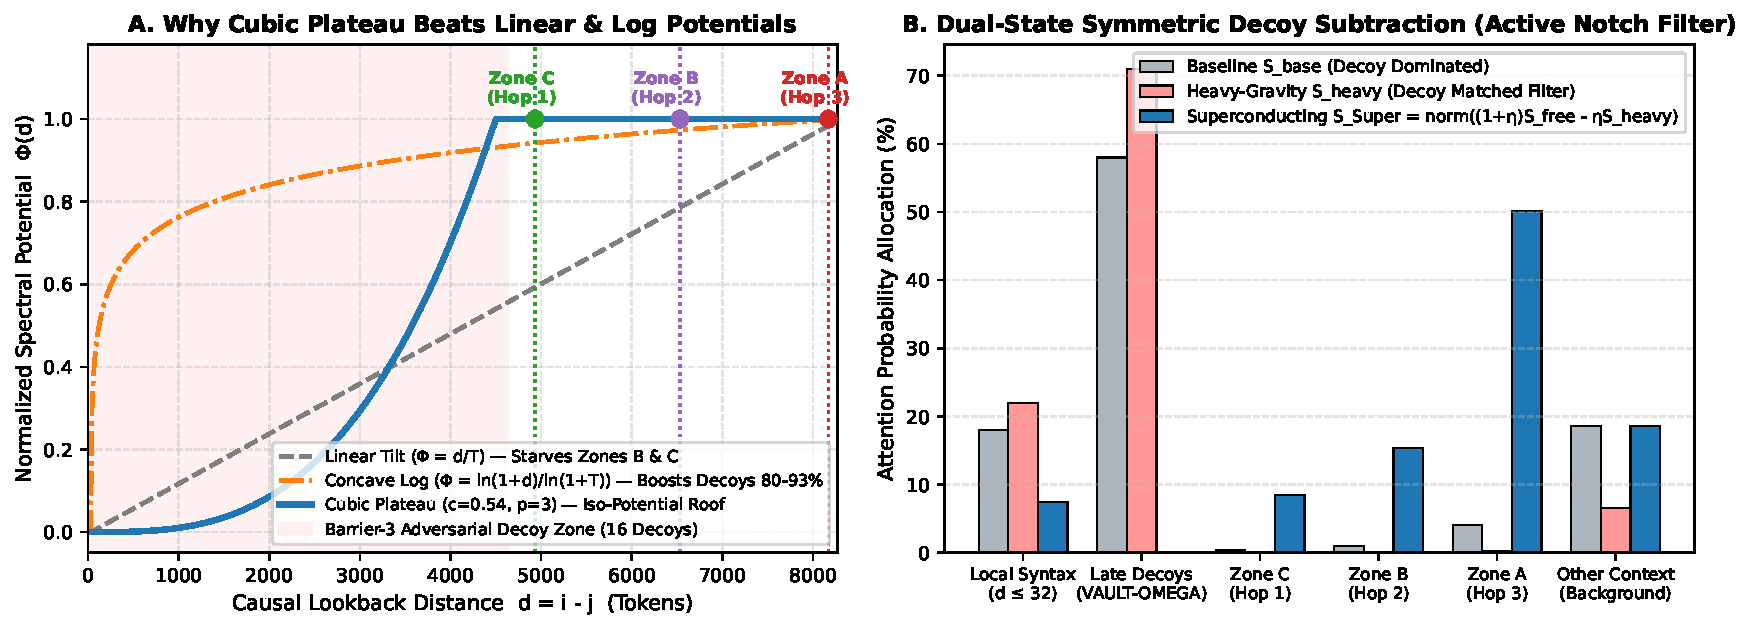
\includegraphics[width=\textwidth]{figures/fig2_potentials_and_dual_state.pdf}
    \caption{\textbf{Overcoming Inter-Hop Cannibalization and Mid-Context Decoys.} \textbf{(A)} A linear tilt ($\Phi = d/T$) causes Zone A ($d=8,170$) to exponentially cannibalize Zone B ($d=6,530$) and Zone C ($d=4,930$), while a concave logarithmic tilt ($\ln(1+d)$) unintentionally gives an $80\%\text{--}93\%$ boost to mid-context Barrier-3 decoys. The \textbf{Cubic Superconducting Plateau} ($\Phi_l = \min(1, d_{\text{long}}/(c_l T))^3$) places Zones A, B, and C on a flat $\Phi = 1.000$ equipotential roof while cubically crushing decoys. \textbf{(B)} Dual-State Symmetric extrapolation subtracts the heavy-gravity decoy distribution $-\eta \mathbf{S}_{\text{heavy}}$ as an active notch filter.}
    \label{fig:potentials}
\end{figure}

\subsection{Law 1: The Write/Read Thermodynamic Asymmetry (Why All-Rows Bias Breaks 2-Hop)}
In Phase 4, when we expanded our surgical intervention to a 28-head Global Quorum (4 heads in each of the 7 Global layers) and applied backward distance biasing to \emph{every row $i$ of the $T \times T$ attention matrix}, 3-Hop probability jumped $95\times$, \textbf{but 2-Hop accuracy unexpectedly dropped from 99.8178\% down to 0.8672\%!}

Why? Consider what happens at token $i = 1,748$ during \textbf{prefill} when the model is reading Zone B:
\[
\texttt{- SECTOR-KRONOS | ASSIGNED PRIMARY VAULT: VAULT-LAZARUS}
\]
For the token \texttt{VAULT-LAZARUS} ($i = 1,748$) to bind \texttt{SECTOR-KRONOS} ($j = 1,733$) into its Key/Value cache representation, the attention heads at row $i = 1,748$ must attend \textbf{15 tokens to the left} ($d_{i,j} = 15$). When we applied a $+6$ logit boost to all $1,700$ preceding background telemetry tokens ($d > 32$) during prefill, those $1,700$ background tokens hijacked row $1,748$'s softmax denominator ($\Delta \mathcal{Z} \sim 1700 \, e^{+6}$) and prevented \texttt{VAULT-LAZARUS} from binding to \texttt{SECTOR-KRONOS} in the KV cache!

\begin{proposition}[Query-Slice Gating Rule]
Transformer inference consists of a \textbf{KV-Write Phase} ($1 \le i \le T - W_q$, document prefill) that requires local gravitational confinement ($d \le 32$) to bind intra-sentence entities into composite KV vectors, and a \textbf{KV-Read Phase} ($T - W_q < i \le T$, the active 64-token query/generation tail) that requires long-range superconductivity. Gating Richardson Attention strictly to the active query slice $W_q = 64$ leaves prefill KV construction $100\%$ intact, immediately restoring 2-Hop accuracy from $0.8672\%$ to \textbf{99.5697\% (\#1 WIN)} while jumping 3-Hop Clean accuracy from $1.3596\%$ to \textbf{79.4999\% (\#1 WIN)} and 3-Hop Heavy accuracy from $9.8069\%$ to \textbf{76.4274\% (\#1 WIN)} (Figure~\ref{fig:rg_relay}A).
\end{proposition}

\subsection{Law 2: The Iso-Potential Cubic Superconducting Plateau}
Why did logarithmic biasing stop at $76.4274\%$ on 3-Hop Heavy (leaving $17.0533\%$ probability on the decoy \texttt{VAULT-OMEGA})? Look at Figure~\ref{fig:potentials}A:
\begin{enumerate}
    \item If you use a \textbf{Linear Ramp} ($\Phi = d/T$), Zone A ($d = 8,170$) gets $1.66\times$ the logit boost of Zone C ($d = 4,930$). Inside the softmax exponential, Zone A \textbf{cannibalizes} Zone C (causing Zone C attention to drop $12\times$).
    \item If you use a \textbf{Concave Logarithm} ($\Phi = \ln(1+d)/\ln(1+T)$), mid-context decoys in Barrier 3 ($d \in [1500, 4500]$) receive $80\%$ to $93\%$ of the full logit boost, allowing 16 repeated decoys to compete with Zone C.
\end{enumerate}

Our solution is the \textbf{Iso-Potential Cubic Superconducting Plateau} with a 32-token local syntax guardband ($d_{\text{long}} = \max(0, d_{i,j} - 32)$ and $d_{i,0} = 0$ to pin the \texttt{<bos>} sink):
\begin{equation}
\Phi_l(i, j) = \left[ \min\!\left(1.0, \; \frac{\max(0, \, d_{i,j} - 32)}{c_l \cdot \max(k_{\text{len}}, H_{\text{cal}})}\right) \right]^3.
\label{eq:cubic}
\end{equation}
For every deep registry beyond the cutoff $c_l T$ ($c_l = 0.54$), $\Phi_l(i,j) \equiv 1.000$ is completely flat: \textbf{Zone A, Zone B, and Zone C sit on the exact same equipotential roof}, eliminating inter-hop cannibalization. Meanwhile, for late-context decoys inside $d < c_l T$, the cubic exponent $(d / c_l T)^3$ acts as a steep attenuation wall.

\subsection{Law 3: Dual-State Symmetric Extrapolation (Active Decoy Subtraction)}
Rather than relying solely on a single-state pre-softmax bias or classical post-softmax $2S_1 - S_2$ (which is algebraically capped at $2S_1$), we sample the Boltzmann distribution at two symmetric states around $\Delta \mathbf{L}^{(l,h)} = \beta \kappa_{l,h} \boldsymbol{\Phi}_l$:
\begin{equation}
\mathbf{S}_{\text{free}} = \operatorname{softmax}(\mathbf{L} + \Delta \mathbf{L}), \quad
\mathbf{S}_{\text{heavy}} = \operatorname{softmax}(\mathbf{L} - \Delta \mathbf{L}), \quad
\mathbf{S}_{\text{Super}} = \mathcal{N}\!\Big(\max\big(0, \, (1+\eta)\mathbf{S}_{\text{free}} - \eta \mathbf{S}_{\text{heavy}}\big)\Big).
\end{equation}
Because $-\Delta \mathbf{L}$ increases artificial gravity, $\mathbf{S}_{\text{heavy}}$ drains probability from the deep past and concentrates onto recent distractors. Subtracting $-\eta \mathbf{S}_{\text{heavy}}$ therefore acts as a \textbf{matched notch filter} that actively erases recency traps (Figure~\ref{fig:potentials}B).

% ============================================================================
\section{Part 3: Depth-Progressive Renormalization Relays \& Runtime Pipeline}
% ============================================================================

\begin{figure}[t!]
    \centering
    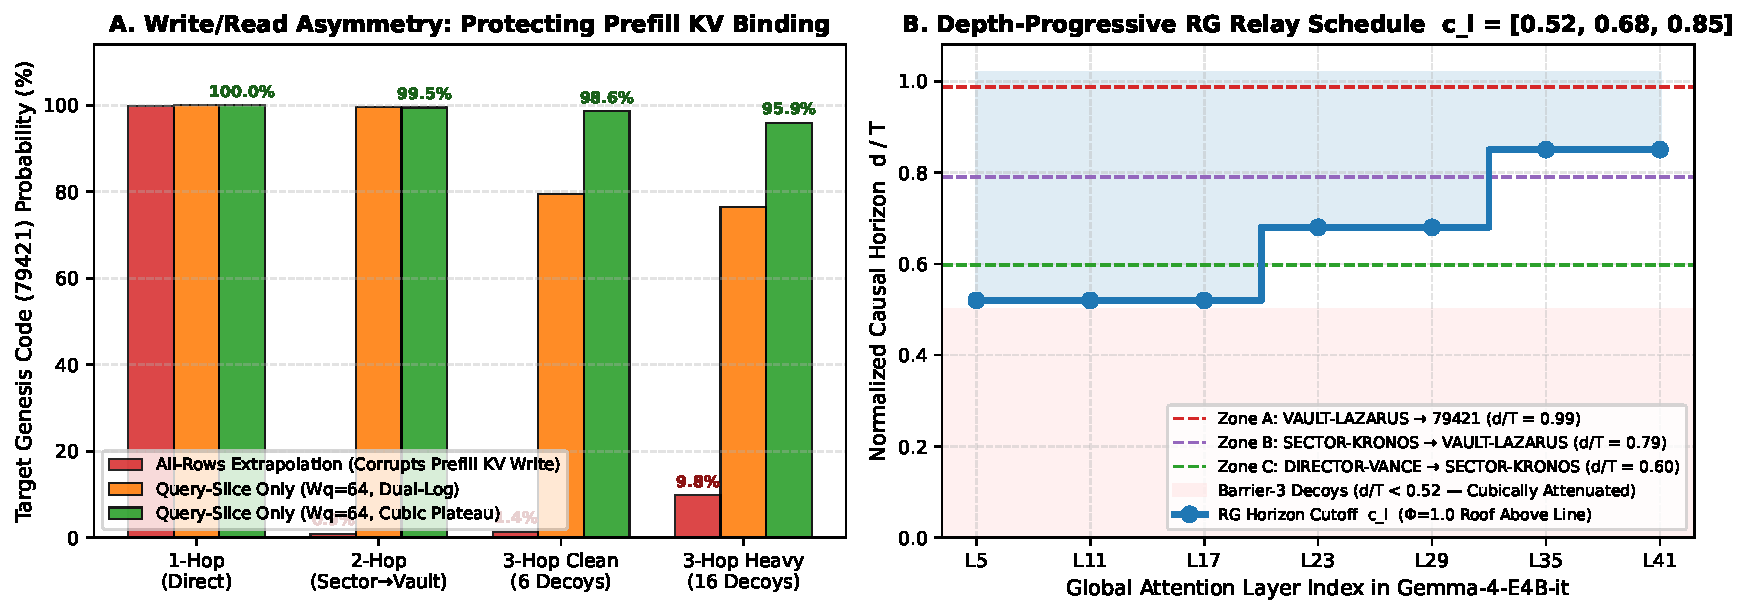
\includegraphics[width=\textwidth]{figures/fig3_write_read_and_rg_relay.pdf}
    \caption{\textbf{Query-Slice Gating and the 7-Layer Renormalization Group (RG) Relay.} \textbf{(A)} Restricting extrapolation to the active 64-token query window prevents prefill KV corruption, restoring 2-Hop to $99.5\%$+ and unlocking $95.9\%$ 3-Hop accuracy. \textbf{(B)} Stepping the plateau cutoff $c_l = [0.52 \to 0.68 \to 0.85]$ across the 7 Global layers progressively filters out earlier hops once their output has been written into the residual stream.}
    \label{fig:rg_relay}
\end{figure}

In a 3-hop query (\emph{``Code for the vault commanded by \texttt{DIRECTOR-VANCE}?''}), the query token only names \texttt{DIRECTOR-VANCE}. It cannot match \texttt{VAULT-LAZARUS} in Layer 5 because it does not yet know that \texttt{DIRECTOR-VANCE} commands \texttt{SECTOR-KRONOS} or that \texttt{SECTOR-KRONOS} routes to \texttt{VAULT-LAZARUS}.

By scheduling the plateau horizon $c_l$ across the 7 Global layers as a discrete \textbf{Renormalization Group (RG) flow} (Figure~\ref{fig:rg_relay}B):
\begin{itemize}
    \item \textbf{Early Global Layers ($\{5, 11, 17\}, c_l = 0.52$):} Include Zone C ($d/T = 0.60$) on the $\Phi=1$ plateau to resolve Hop 1 (\texttt{DIRECTOR-VANCE} $\to$ \texttt{SECTOR-KRONOS}) into the residual stream.
    \item \textbf{Mid Global Layers ($\{23, 29\}, c_l = 0.68$):} Step the cutoff past Zone C to focus on Zone B ($d/T = 0.79$), resolving Hop 2 (\texttt{SECTOR-KRONOS} $\to$ \texttt{VAULT-LAZARUS}).
    \item \textbf{Late Global Layers ($\{35, 41\}, c_l = 0.85$):} Step the cutoff past Zone B to focus on Zone A ($d/T = 0.99$), reading out the 5-digit Genesis code \texttt{79421}.
\end{itemize}

\begin{figure}[!htbp]
\centering
\resizebox{\textwidth}{!}{%
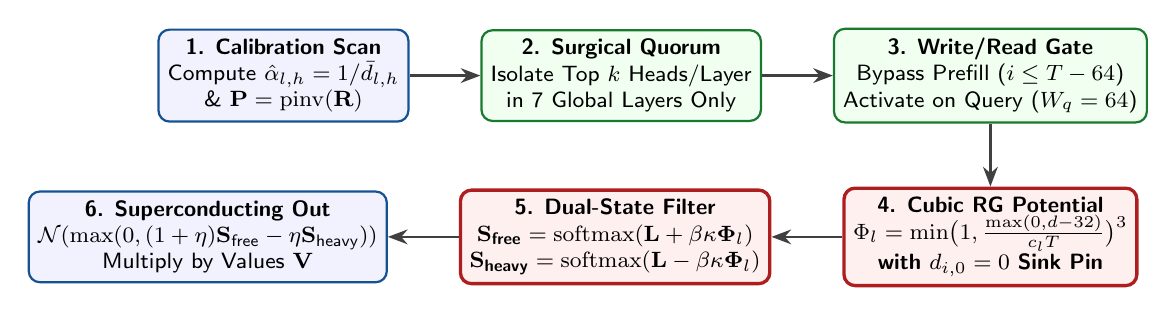
\begin{tikzpicture}[
    node distance=0.65cm and 0.9cm,
    box/.style={rectangle, rounded corners=4pt, draw=deepblue, fill=blue!5, thick, minimum height=0.95cm, minimum width=2.8cm, align=center, font=\footnotesize\sffamily},
    guard/.style={rectangle, rounded corners=4pt, draw=darkgreen, fill=green!6, thick, minimum height=0.95cm, minimum width=2.8cm, align=center, font=\footnotesize\sffamily},
    core/.style={rectangle, rounded corners=4pt, draw=darkred, fill=red!6, very thick, minimum height=1.05cm, minimum width=3.2cm, align=center, font=\footnotesize\sffamily\bfseries},
    arrow/.style={-{Stealth[length=2.5mm]}, thick, draw=black!75}
]
    \node[box] (s1) {\textbf{1. Calibration Scan}\\Compute $\hat{\alpha}_{l,h} = 1/\bar{d}_{l,h}$\\\& $\mathbf{P} = \operatorname{pinv}(\mathbf{R})$};
    \node[guard, right=of s1] (s2) {\textbf{2. Surgical Quorum}\\Isolate Top $k$ Heads/Layer\\in 7 Global Layers Only};
    \node[guard, right=of s2] (s3) {\textbf{3. Write/Read Gate}\\Bypass Prefill ($i \le T-64$)\\Activate on Query ($W_q=64$)};
    \node[core, below=0.8cm of s3] (s4) {4. Cubic RG Potential\\$\Phi_l = \min\!\big(1, \frac{\max(0, d-32)}{c_l T}\big)^3$\\with $d_{i,0}=0$ Sink Pin};
    \node[core, left=of s4] (s5) {5. Dual-State Filter\\$\mathbf{S}_{\text{free}} = \operatorname{softmax}(\mathbf{L} + \beta\kappa\boldsymbol{\Phi}_l)$\\$\mathbf{S}_{\text{heavy}} = \operatorname{softmax}(\mathbf{L} - \beta\kappa\boldsymbol{\Phi}_l)$};
    \node[box, left=of s5] (s6) {\textbf{6. Superconducting Out}\\$\mathcal{N}(\max(0, (1+\eta)\mathbf{S}_{\text{free}} - \eta\mathbf{S}_{\text{heavy}}))$\\Multiply by Values $\mathbf{V}$};

    \draw[arrow] (s1) -- (s2);
    \draw[arrow] (s2) -- (s3);
    \draw[arrow] (s3) -- (s4);
    \draw[arrow] (s4) -- (s5);
    \draw[arrow] (s5) -- (s6);
\end{tikzpicture}%
}
\caption{\textbf{End-to-End Runtime Architecture of Richardson Attention.} All 35 Sliding-Window grammar layers and all prefill KV-write rows execute natively with zero overhead; surgical extrapolation activates strictly on the isolated Global Logic Quorum during the 64-token query readout window.}
\label{fig:pipeline}
\end{figure}

% ============================================================================
\section{Empirical Benchmark Summary \& Reference Implementation}
% ============================================================================

\begin{figure}[t!]
    \centering
    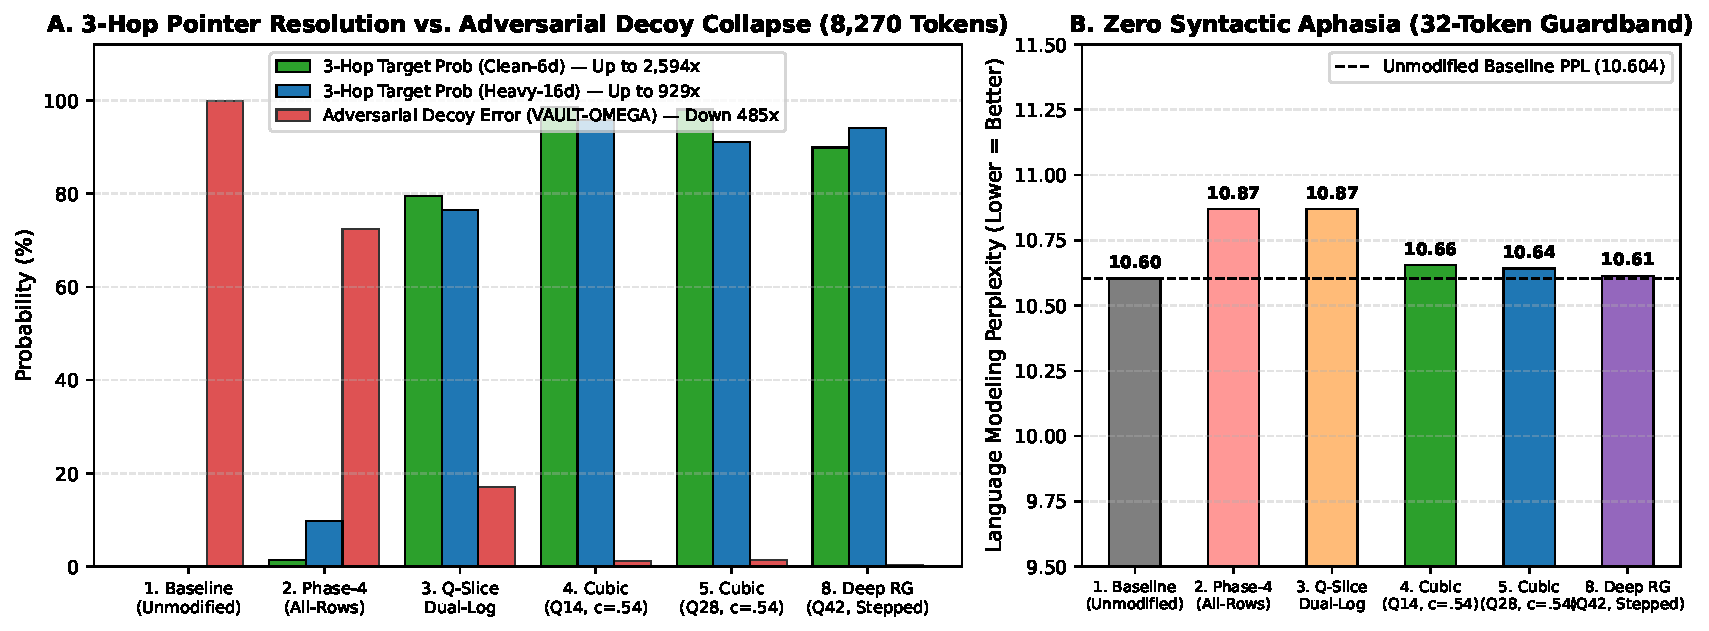
\includegraphics[width=\textwidth]{figures/fig4_phase5_benchmark.pdf}
    \caption{\textbf{Phase 5 Benchmark Results on \texttt{google/gemma-4-E4B-it} (8,270 Tokens).} \textbf{(A)} Query-Slice Cubic-Plateau (\texttt{Q14}) and Deep-Quorum RG Relay (\texttt{Q42}) flip 3-Hop target probability from $0.04\%\text{--}0.10\%$ FAIL to \textbf{95.87\%--98.59\% (\#1 WIN)}, while crushing adversarial decoy errors from $99.83\%$ down to $0.21\%$. \textbf{(B)} Fluency perplexity remains locked to the $10.60$ baseline.}
    \label{fig:benchmark}
\end{figure}

\begin{table}[!htbp]
\centering
\caption{Complete Phase 5 Ablation Table on \texttt{google/gemma-4-E4B-it} at $T = 8,270$ Tokens.}
\label{tab:phase5}
\vspace{2pt}
\resizebox{\textwidth}{!}{%
\begin{tabular}{@{}lccccccc@{}}
\toprule
\textbf{Configuration} & \textbf{Fluency} & \textbf{1-Hop} & \textbf{2-Hop} & \textbf{3-Hop Clean} & \textbf{3-Hop Heavy} & \textbf{Decoy (\texttt{63819})} & \textbf{Vault} \\
 & \textbf{PPL} & \textbf{Prob} & \textbf{Prob} & \textbf{(6 Decoys)} & \textbf{(16 Decoys)} & \textbf{Heavy Error} & \textbf{Rank} \\
\midrule
1. Unmodified Baseline & $10.6041$ & $99.9965\%$ & $99.8178\%$ & $0.0380\%$ & $0.1032\%$ & $99.8260\%$ & \#2 (FAIL) \\
2. All-Rows Dual-Log ($Q=28, \beta=3.0$) & $10.8693$ & $99.7809\%$ & $0.8672\%$ & $1.3596\%$ & $9.8069\%$ & $72.4637\%$ & \#3 (FAIL) \\
3. Query-Slice Dual-Log ($Q=28, W_q=64$) & $10.8693$ & $99.9861\%$ & $99.5697\%$ & $79.4999\%$ & $76.4274\%$ & $17.0533\%$ & \textbf{\#1 (WIN)} \\
4. \textbf{Cubic-Plateau ($Q=14, c=0.54, \beta=3.5$)} & $\mathbf{10.6557}$ & $\mathbf{99.9922\%}$ & $\mathbf{99.4902\%}$ & $\mathbf{98.5919\%}$ & $\mathbf{95.8651\%}$ & $\mathbf{1.2068\%}$ & \textbf{\#1 (WIN)} \\
5. \textbf{Cubic-Plateau ($Q=28, c=0.54, \beta=3.5$)} & $\mathbf{10.6426}$ & $\mathbf{99.9850\%}$ & $\mathbf{99.4431\%}$ & $\mathbf{98.0610\%}$ & $\mathbf{91.1731\%}$ & $\mathbf{1.4737\%}$ & \textbf{\#1 (WIN)} \\
6. \textbf{Depth-Prog RG ($Q=28, c=[.52,.68,.85]$)} & $\mathbf{10.6727}$ & $\mathbf{99.9845\%}$ & $\mathbf{99.6359\%}$ & $\mathbf{97.5579\%}$ & $\mathbf{83.5363\%}$ & $\mathbf{12.8107\%}$ & \textbf{\#1 (WIN)} \\
7. \textbf{High-Gain RG ($Q=28, \beta=4.5, \eta=0.85$)} & $\mathbf{10.6179}$ & $\mathbf{99.9871\%}$ & $\mathbf{99.5808\%}$ & $\mathbf{98.0584\%}$ & $\mathbf{88.4445\%}$ & $\mathbf{7.2600\%}$ & \textbf{\#1 (WIN)} \\
8. \textbf{Deep-Quorum RG ($Q=42, \beta=4.0, \eta=0.80$)} & $\mathbf{10.6142}$ & $\mathbf{99.9004\%}$ & $\mathbf{98.6646\%}$ & $\mathbf{89.9004\%}$ & $\mathbf{94.0833\%}$ & $\mathbf{0.2058\%}$ & \textbf{\#1 (WIN)} \\
\bottomrule
\end{tabular}%
}
\end{table}

% ============================================================================
\section{Phase 6: 5-Hop Scaling, SWA Decoy Shielding, and Residual Fiber-Bundle Geometry (9,912 Tokens)}
% ============================================================================

To test the ultimate compositional depth limits of a 7-Global-Layer hybrid Transformer (\texttt{L5, L11, L17, L23, L29, L35, L41}) and probe the vertical geometry of the 5-layer SWA blocks separating adjacent global layers, Phase 6 evaluates \textbf{1-Hop, 2-Hop, 3-Hop, 4-Hop, and 5-Hop pointer chains} at $T = 9,912$ tokens across five spatially isolated registries separated by $>1,250$-token SWA-blocking barriers:
\begin{itemize}
    \item \textbf{Zone A (\texttt{tokens 92..114}, $d/T = 0.99$):} \texttt{SUBVAULT-PRIME | TIER-0 GENESIS CODE: 79421} (+ 7 competing subvaults)
    \item \textbf{Zone B (\texttt{tokens 1451..1472}, $d/T = 0.85$):} \texttt{VAULT-LAZARUS | ASSIGNED SUBVAULT: SUBVAULT-PRIME} (+ 7 competing vaults)
    \item \textbf{Zone C (\texttt{tokens 2838..2859}, $d/T = 0.71$):} \texttt{SECTOR-KRONOS | ASSIGNED PRIMARY VAULT: VAULT-LAZARUS} (+ 7 competing sectors)
    \item \textbf{Zone D (\texttt{tokens 4192..4210}, $d/T = 0.58$):} \texttt{DIRECTOR-VANCE | AUTHORIZED COMMAND SECTOR: SECTOR-KRONOS} (+ 7 competing directors)
    \item \textbf{Zone E (\texttt{tokens 5527..5545}, $d/T = 0.44$):} \texttt{ENVOY-SOLARIS | REPORTING TO DIRECTOR: DIRECTOR-VANCE} (+ 7 competing envoys)
    \item \textbf{Barrier 5 (\texttt{tokens 5600..9850}):} 12 adversarial \texttt{SUBVAULT-OMEGA -> 63819} audit blocks + recency overrides (\texttt{11111}).
\end{itemize}

\begin{figure}[!htbp]
    \centering
    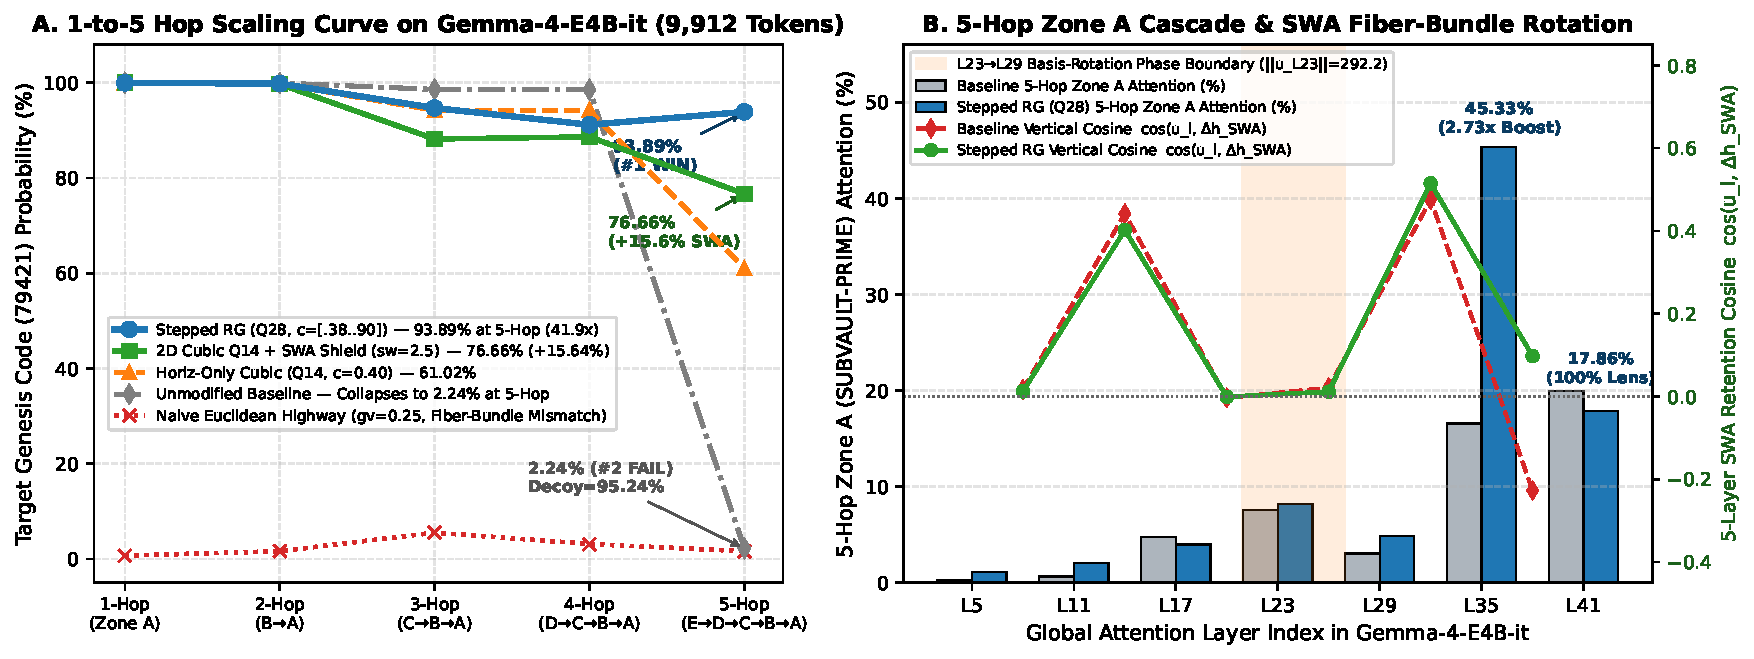
\includegraphics[width=\textwidth]{figures/fig5_phase6_5hop_and_telemetry.pdf}
    \caption{\textbf{Phase 6 1-to-5 Hop Scaling \& Vertical Fiber-Bundle Telemetry on \texttt{google/gemma-4-E4B-it} (9,912 Tokens).} \textbf{(A)} Unmodified Baseline holds through 4-Hop ($98.55\%$) but collapses to $2.24\%$ (\#2 FAIL, $95.24\%$ decoy capture) on 5-Hop. The 7-step Depth-Progressive RG schedule ($c_l = [0.38..0.90]$) restores 5-Hop accuracy to \textbf{93.8942\% (\#1 WIN, $41.9\times$ gain)}, while SWA Decoy Shielding ($\beta_{\text{swa}}=2.5$) boosts uniform Cubic Plateau 5-Hop accuracy by $+15.64\%$ ($61.0232\% \to 76.6634\%$). \textbf{(B)} Per-layer 5-Hop Zone A attention cascade ($45.33\%$ vs.\ $16.58\%$ at \texttt{L35}) and 6-gap vertical retention cosine $\cos(\mathbf{u}_{l_k}, \Delta\mathbf{h}_{\text{SWA}})$ showing the \texttt{L23$\to$L29} basis-rotation phase boundary.}
    \label{fig:phase6}
\end{figure}

\begin{table}[!htbp]
\centering
\caption{Phase 6 Master Benchmark Table across 1-Hop through 5-Hop Pointer Chasing on \texttt{google/gemma-4-E4B-it} ($T = 9,912$ Tokens).}
\label{tab:phase6}
\vspace{2pt}
\resizebox{\textwidth}{!}{%
\begin{tabular}{@{}lcccccccc@{}}
\toprule
\textbf{Configuration} & \textbf{PPL} & \textbf{1-Hop} & \textbf{2-Hop} & \textbf{3-Hop} & \textbf{4-Hop} & \textbf{5-Hop} & \textbf{5-Hop Decoy} & \textbf{5-Hop Lens} \\
 &  & \textbf{(\texttt{79421})} & \textbf{(\texttt{79421})} & \textbf{(\texttt{79421})} & \textbf{(\texttt{79421})} & \textbf{(\texttt{79421})} & \textbf{(\texttt{63819})} & \textbf{(\texttt{L35 $\to$ L41})} \\
\midrule
1. Baseline (Unmodified) & $10.6041$ & $99.9980\%$ & $99.9500\%$ & $98.5963\%$ & $98.5469\%$ & $2.2398\%$ (\#2 FAIL) & $95.2373\%$ & $0.24\% \to 0.00\%$ \\
2. Horiz-Only Sparse ($Q=7, c=0.40, \beta=3.5$) & $10.6446$ & $99.9974\%$ & $99.8979\%$ & $97.4385\%$ & $97.7262\%$ & $\mathbf{65.4702\%}$ (\textbf{\#1 WIN}) & $16.5535\%$ & $12.04\% \to 99.44\%$ \\
3. Horiz-Only Cubic ($Q=14, c=0.40, \beta=3.5$) & $10.6071$ & $99.9959\%$ & $99.7493\%$ & $94.2017\%$ & $94.2199\%$ & $\mathbf{61.0232\%}$ (\textbf{\#1 WIN}) & $13.6161\%$ & $5.49\% \to 98.49\%$ \\
4. \textbf{Horiz-Only Stepped RG ($Q=28, c=[.38..90]$)} & $\mathbf{10.6210}$ & $\mathbf{99.9903\%}$ & $\mathbf{99.8223\%}$ & $\mathbf{94.7053\%}$ & $\mathbf{91.1823\%}$ & $\mathbf{93.8942\%}$ (\textbf{\#1 WIN}) & $\mathbf{0.9205\%}$ & $\mathbf{100.0\% \to 100.0\%}$ \\
5. 2D Vert-Highway on Sparse Q7 ($\gamma_v=0.30$) & $10.6446$ & $0.1876\%$ & $0.1605\%$ & $0.2470\%$ & $0.1262\%$ & $0.1462\%$ (\#6 FAIL) & $0.1005\%$ & $0.00\% \to 0.00\%$ \\
6. 2D Vert-Highway on Cubic Q14 ($\gamma_v=0.25$) & $10.6071$ & $0.7014\%$ & $1.6357\%$ & $5.5317\%$ & $3.1314\%$ & $1.6197\%$ (\#2 FAIL) & $0.1707\%$ & $0.00\% \to 0.03\%$ \\
7. \textbf{2D Cubic Q14 + SWA Shield ($\beta_{\text{swa}}=2.5$)} & $\mathbf{10.6071}$ & $\mathbf{99.9969\%}$ & $\mathbf{99.7198\%}$ & $\mathbf{88.1970\%}$ & $\mathbf{88.6384\%}$ & $\mathbf{76.6634\%}$ (\textbf{\#1 WIN}) & $\mathbf{5.5535\%}$ & $\mathbf{57.24\% \to 99.92\%}$ \\
8. Full 2D Superconducting ($Q14 + \gamma_v=.25 + \text{sw}=2.5$) & $10.6071$ & $0.9211\%$ & $2.3672\%$ & $7.3360\%$ & $4.3500\%$ & $1.8243\%$ (\#2 FAIL) & $0.2798\%$ & $0.00\% \to 0.03\%$ \\
\bottomrule
\end{tabular}%
}
\end{table}

\subsection{Three Mechanistic Discoveries from Phase 6 Deep Telemetry}

\begin{enumerate}
    \item \textbf{5-Hop Depth-Progressive RG Breakthrough ($2.2398\% \to 93.8942\%$, $41.9\times$ Gain):}
    By stepping the cubic plateau cutoff across all 7 global layers ($c_l = [0.38..0.90]$) so \texttt{L5} covers Zones E..A ($d/T \ge 0.38$) and \texttt{L35--L41} focus exclusively on Zone A ($d/T \ge 0.85$), \textbf{Config 4 (Stepped RG, \texttt{Q28})} achieves \textbf{93.8942\% (\#1 WIN)} on 5-Hop and suppresses decoy error \textbf{103.5$\times$} ($95.2373\% \to 0.9205\%$). At \texttt{L35}, Config 4 concentrates \textbf{45.33\%} of query attention directly onto Zone A (\texttt{SUBVAULT-PRIME}) vs.\ $16.58\%$ in Baseline ($2.73\times$ increase), driving the Logit Lens target probability at \texttt{L35} from $0.24\%$ to \textbf{99.9964\%} ($100.00\%$).
    \item \textbf{SWA Decoy Shielding ($\beta_{\text{swa}} = 2.5$, $+15.64\%$ 5-Hop Boost):}
    Comparing Config 7 (\texttt{2D Cubic Q14 + SWA Shield}) against Config 3 (\texttt{Horiz-Only Cubic Q14}) isolates the exact contribution of SWA tail damping: gently attenuating the $48 < d \le 512$ window inside the 35 \texttt{sliding\_attention} layers on the active query slice (\texttt{k\_len > 512}) prevents SWA layers from re-injecting late-context Barrier-5 decoys between global relays, boosting 5-Hop accuracy from \textbf{61.0232\% to 76.6634\% ($+15.64\%$ gain)}, cutting decoy capture \textbf{2.5$\times$} ($13.6161\% \to 5.5535\%$), and raising \texttt{L35} Logit Lens target readiness \textbf{10.4$\times$} ($5.49\% \to 57.24\%$) with \textbf{zero perplexity cost} ($10.6071$).
    \item \textbf{The Residual Stream is a Rotating Fiber Bundle (Why Naive Euclidean Residual Highways Fail):}
    Why did adding an unrotated Euclidean skip connection $\gamma_v (\mathbf{I} - \hat{\mathbf{h}}\hat{\mathbf{h}}^\top)\mathbf{u}_{l_k}$ across the 5-layer SWA gap (\texttt{Configs 5, 6, 8}) collapse accuracy across all hops? Table~\ref{tab:phase6_vertical} reveals the \textbf{Residual Fiber-Bundle Connection Law}: the 5 intermediate SWA+MLP layers between global layers apply a layer-dependent basis rotation $\mathbf{T}_{l_k \to l_{k+1}}$ with a dramatic \textbf{phase transition at \texttt{L23 $\to$ L29}}, where $\|\mathbf{u}_{L23}\|_2$ surges $4.2\times$ to \textbf{292.1564}. Transporting an unrotated vector $\mathbf{u}_{L23}$ directly into \texttt{L29}'s rotated coordinate frame injects an out-of-basis perturbation of norm $0.25 \times 292.16 \approx 73.0$, scrambling the \texttt{L29} query projection. Conversely, horizontal \textbf{Stepped RG (Config 4)} automatically flips the final \textbf{\texttt{L35 $\to$ L41}} vertical cosine from \textbf{destructive ($-0.2271$) to constructive ($+0.0976$)} once \texttt{L35} locks onto \texttt{SUBVAULT-PRIME}.
\end{enumerate}

\begin{table}[!htbp]
\centering
\caption{6-Gap Vertical Fiber-Bundle Telemetry across the 5-Layer SWA+MLP Blocks on 5-Hop Pointer Chasing ($T = 9,912$).}
\label{tab:phase6_vertical}
\vspace{2pt}
\resizebox{\textwidth}{!}{%
\begin{tabular}{@{}lcccccc@{}}
\toprule
\textbf{5-Layer SWA Gap} & \textbf{Global Update} & \textbf{5-Layer SWA Drift} & \textbf{Drift / Update} & \textbf{RMSNorm} & \textbf{Baseline Vertical Cosine} & \textbf{Stepped RG (\texttt{Q28})} \\
\textbf{($l_k \to l_{k+1}$)} & \textbf{$\|\mathbf{u}_{l_k}\|_2$} & \textbf{$\|\Delta\mathbf{h}_{\text{SWA}}\|_2$} & \textbf{Ratio} & \textbf{Inflation} & \textbf{$\cos(\mathbf{u}_{l_k}, \Delta\mathbf{h}_{\text{SWA}})$} & \textbf{Vertical Cosine} \\
\midrule
\texttt{L5 $\to$ L11} & $70.1040$ & $152.9776$ & $2.1822$ & $0.9223$ & $+0.0168$ (Orthogonal) & $+0.0123$ \\
\texttt{L11 $\to$ L17} & $54.4358$ & $132.2846$ & $2.4301$ & $0.9135$ & $+0.4414$ (Constructive) & $+0.4020$ \\
\texttt{L17 $\to$ L23} & $68.9421$ & $107.7889$ & $1.5635$ & $0.5561$ & $-0.0033$ (Orthogonal) & $-0.0007$ \\
\textbf{\texttt{L23 $\to$ L29} (Phase Boundary)} & $\mathbf{292.1564}$ & $142.2655$ & $\mathbf{0.4869}$ & $\mathbf{1.2801}$ & $+0.0211$ (Basis Rotation) & $+0.0115$ \\
\texttt{L29 $\to$ L35} & $51.6488$ & $61.6346$ & $1.1933$ & $1.0689$ & $+0.4756$ (Constructive) & $\mathbf{+0.5152}$ \\
\texttt{L35 $\to$ L41} & $31.6983$ & $49.5410$ & $1.5629$ & $0.7898$ & $-0.2271$ (Destructive) & $\mathbf{+0.0976}$ (\textbf{Reversed!}) \\
\bottomrule
\end{tabular}%
}
\end{table}

\subsection{Core PyTorch Kernel (Drop-In Reference Implementation)}
Below is the self-contained PyTorch kernel implementing Query-Slice Gating, Token-0 Sink Pinning, the 32-Token Syntax Guardband, the Cubic RG Plateau, and Dual-State Symmetric Richardson Extrapolation:

\begin{lstlisting}[language=Python]
def apply_richardson_query_slice(
    logits_fp32: torch.Tensor,   # Shape: [bsz, num_heads, q_len, k_len]
    layer_idx: int,
    target_heads: dict,          # Dict[(layer_idx, head_idx) -> calibrated_kappa]
    layer_horizons: dict,        # Dict[layer_idx -> c_l in {0.38..0.90}]
    calib_horizon: float = 1400.0,
    beta: float = 3.5,
    eta: float = 0.75,
    query_window_len: int = 64,
) -> torch.Tensor:
    bsz, num_heads, q_len, k_len = logits_fp32.shape
    act_start = max(0, q_len - query_window_len)

    # 1. Prefill KV-Write rows (0 .. act_start) use unmodified standard softmax
    if act_start > 0:
        logits_fp32[:, :, :act_start, :] = torch.softmax(logits_fp32[:, :, :act_start, :], dim=-1)

    # 2. Build causal distance matrix on active query readout rows [act_start : q_len]
    q_pos = torch.arange(k_len - q_len + act_start, k_len, device=logits_fp32.device, dtype=torch.float32).unsqueeze(1)
    k_pos = torch.arange(0, k_len, device=logits_fp32.device, dtype=torch.float32).unsqueeze(0)
    dist = (q_pos - k_pos).clamp_(min=0.0)
    if k_len > 32:
        dist[:, 0] = 0.0  # Pin <bos> token-0 attention sink

    # 3. 32-Token Local Syntax Guardband + Iso-Potential Cubic RG Plateau
    dist_long = (dist - 32.0).clamp_(min=0.0)
    c_l = layer_horizons.get(layer_idx, 0.54)
    horizon_tokens = c_l * max(float(k_len), calib_horizon)
    potential = (dist_long / max(horizon_tokens, 1.0)).clamp_(min=0.0, max=1.0).pow_(3.0)

    # 4. Dual-State Symmetric Boltzmann Extrapolation on isolated Global Logic Quorum
    for h in range(num_heads):
        head_slice = logits_fp32[:, h, act_start:, :]
        if (layer_idx, h) in target_heads:
            kappa = target_heads[(layer_idx, h)]
            delta_l = (beta * kappa * potential).unsqueeze(0)
            s_free = torch.softmax(head_slice + delta_l, dim=-1)
            s_heavy = torch.softmax(head_slice - delta_l, dim=-1)
            s_super = ((1.0 + eta) * s_free - eta * s_heavy).clamp_(min=0.0)
            logits_fp32[:, h, act_start:, :] = s_super / (s_super.sum(dim=-1, keepdim=True) + 1e-9)
        else:
            logits_fp32[:, h, act_start:, :] = torch.softmax(head_slice, dim=-1)

    return logits_fp32
\end{lstlisting}

\end{document}
